\documentclass{article}
\usepackage[T1]{fontenc}
\usepackage[utf8]{inputenc}
\usepackage[polish]{babel}
\usepackage{amsmath}
\usepackage{url}
\usepackage{graphicx}
 \usepackage{float}
 \usepackage{pgfplots}
\pgfplotsset{compat=1.18}
%{Informatyka stosowana 2022, I st., semestr VI}


\author{
	{Dominik Gałkowski, 247659} \\
	{Jan Śladowski, 247806}\\ 
{Prowadzący: dr inż. Marcin Kacprowicz}
}

\title{Komputerowe systemy rozpoznawania 2024/2025\\Projekt 2. Podsumowania lingwistyczne relacyjnych baz danych}
\begin{document}
\maketitle 

\section{Cel}
Celem projektu jest stworzenie aplikacji, której główną funkcjonalnością
jest lingwistyczna agregacja zawartości wybranego zbioru danych. Ma ona za zadanie generowanie podsumowań lingwistycznych dla wybranych przez użytkownika kwantyfikatorów, sumaryzatorów i kwalifikatorów dla różnych atrybutów. Analiza otrzymanych wyników polega na określeniu, znaczenia wybranych kwantyfikatorów, sumaryzatorów, kwalifikatorów oraz miar ich jakości dla wiarygodności i jakości otrzymanych podsumowań lingwistycznych. Przykładowe podsumowanie to, np. większość pomiarów ma wysokie ciśnienie.


\section{Baza danych, zmienne lingwistyczne, kwantyfikatory lingwistyczne}

\subsection{Charakterystyka podsumowywanej bazy danych}
W tym projekcie został wykorzystany zbiór danych zapisany w pliku w formacie .csv, na podstawie którego utworzono bazę danych - PostgresSQL. Baza danych o nazwie World Weather Repository zawiera różnego rodzaju pomiary danych atmosferycznych, np. temperatura lub prędkość wiatru. \cite{baza} Użteczność bazy jest określona na stronie Kaggle jako 10.0, a dane z niej są wykorzystywane do prognozowanie pogody oraz analizy klimatu na różnych kontynentach. Baza jest nabieżąco aktualizowana, natomiast na dzień 18.05.2025r. składa się z 62603 rekordów. 

Zmiennym lingwistycznym przypisuje się znaczenie ze względu na potrzebę lepszej interpretowalności danych przez użytkowników. Ludzie rzadko reagują na dokładne wartości (np. 1033.8 mb ciśnienia), natomiast określenie „wysokie ciśnienie” pozwala im intuicyjnie rozumieć sytuację pogodową. Stąd istnieje zapotrzebowanie na „przekładanie” danych formalnych na język naturalny. \\
Podmiotem podsumowań jest pomiar atmosferyczny, z bazy World Weather Repository wybrano 10 atrybutów, które zostaną rozmyte, są to następujące kolumny: last\_updated, temperature\_celsius, wind\_kph, pressure\_mb, humidity, visibility\_km, uv\_index, air\_quality\_Carbon\_Monoxide,  \\air\_quality\_Nitrogen\_dioxide, air\_quality\_gb\_defra\_index \\
Dokładne opisy atrybutów znajdują się w załączniku pod nazwą załącznik1.pdf.

\subsection{Zmienne lingwistyczne (atrybuty/własności obiektów)}
Poniżej zostały zaprezentowane zmienne lingwistyczne dla atrybutów opisanych w sekcji 2.1 oraz ich wzory analityczne. W każdym z poniższych wzorów \(L_x\) to zmienna ligwistyczna, $\mathcal{L}_x$ - nazwa zmiennej lingwistycznej , \(H_x\) zbiór możliwych przyjmowanych wartości, \(X_x\) - przestrzeń rozważań, \(x\) - numer kolejnej zmiennej lingwistycznej. 
\begin{enumerate}
    \item last\_updated
        \begin{equation}
            L_1 = \langle \mathcal{L}_1, H_1, \mathcal{X}_1 \rangle
        \end{equation}
        gdzie: $\mathcal{L}_1$ – pora dnia, $H_1$ – \{nocna, poranna, południowa, popołudniowa, wieczorna\}, $\mathcal{X}_1 = [0, 24]$. \\
        Poniżej wzory dla wszystkich możliwych etykiet.
        \begin{equation}
            \mu_{\text{nocna}}(x) =
            \begin{cases}
            \frac{7 - x}{3}, & x \in (4, 7) \\
            1, & x \in [0, 4] \\
            \frac{x - 21}{3}, & x \in [21, 24) \\
            0, & \text{w przeciwnym razie} \\
            \end{cases}
        \end{equation}

        \begin{equation}
            \mu_{\text{poranna}}(x) =
            \begin{cases}
            \frac{x - 4}{3}, & x \in (4, 7) \\
            1, & x \in [7, 9] \\
            \frac{12 - x}{3}, & x \in (9, 12) \\
            0, & \text{w przeciwnym razie} \\
            \end{cases}
        \end{equation}

        \begin{equation}
            \mu_{\text{południowa}}(x) =
            \begin{cases}
            \frac{x - 9}{3}, & x \in (9, 12) \\
            1, & x \in [12, 13] \\
            \frac{16 - x}{3}, & x \in (13, 16) \\
            0, & \text{w przeciwnym razie} \\
            \end{cases}
        \end{equation}

        \begin{equation}
            \mu_{\text{popołudniowa}}(x) =
            \begin{cases}
            \frac{x - 13}{3}, & x \in (13, 16) \\
            1, & x \in [16, 17] \\
            \frac{20 - x}{3}, & x \in (17, 20) \\
            0, & \text{w przeciwnym razie} \\
             \end{cases}
        \end{equation}

        \begin{equation}
            \mu_{\text{wieczorna}}(x) =
            \begin{cases}
            \frac{x - 17}{3}, & x \in (17, 20) \\
            1, & x \in [20, 21] \\
            \frac{24 - x}{3}, & x \in (21, 24) \\
            0, & \text{w przeciwnym razie} \\
            \end{cases}
        \end{equation} 
        
Wykres funkcji przynależności znajduje się w załączniku pod nazwą img/day.png.
    
    \item temperature\_celsius
        \begin{equation}
            L_2 = \langle \mathcal{L}_2, H_2, \mathcal{X}_2 \rangle
        \end{equation}
        gdzie: $\mathcal{L}_2$ – temperatura, $H_2$ – \{bardzo zimna, zimna, umiarkowana, ciepła, gorąca\}, $\mathcal{X}_2 = [-25, 50]$. \\
        Poniżej wzory dla wszystkich możliwych etykiet.
                \begin{equation}
                   \mu_{\text{bardzo\_zimna}}(x) =
                    \begin{cases}
                    1, & x \in [-25, -15] \\
                    \frac{-5 - x}{10}, & x \in (-15, -5) \\
                    0, & \text{w przeciwnym razie}
                    \end{cases}
                \end{equation}
                
                \begin{equation}
                   \mu_{\text{zimna}}(x) =
                    \begin{cases}
                    \frac{x + 10}{10}, & x \in (-15, -5) \\
                    1, & x \in [-5, 0] \\
                    \frac{10 - x}{10}, & x \in (0, 10) \\
                    0, & \text{w przeciwnym razie}
                    \end{cases}
                \end{equation}

                \begin{equation}
                    \mu_{\text{umiarkowana}}(x) =
                    \begin{cases}
                    \frac{x}{10}, & x \in (0, 10) \\
                    1, & x \in [10, 15] \\
                    \frac{20 - x}{10}, & x \in (15, 25) \\
                    0, & \text{w przeciwnym razie}
                    \end{cases}
                \end{equation}

                \begin{equation}
                    \mu_{\text{ciepła}}(x) =
                    \begin{cases}
                    \frac{x - 15}{10}, & x \in (15, 25) \\
                    1, & x \in [25, 30] \\
                    \frac{30 - x}{10}, & x \in (30, 40) \\
                    0, & \text{w przeciwnym razie}
                    \end{cases}
                \end{equation}

                \begin{equation}
                    \mu_{\text{gorąca}}(x) =
                    \begin{cases}
                    \frac{x - 30}{10}, & x \in (30, 40] \\
                    1, & x \in 40, 50] \\
                    0, & \text{w przeciwnym razie}
                    \end{cases}
                \end{equation}

Wykres funkcji przynależności znajduje się w załączniku pod nazwą img/temp.png.

    \item wind\_kph
        \begin{equation}
            L_3 = \langle \mathcal{L}_3, H_3, \mathcal{X}_3 \rangle
        \end{equation}
        gdzie: $\mathcal{L}_3$ – wiatr, $H_3$ – \{słaby, umiarkowany, silny, bardzo silny, gwałtowny\}, $\mathcal{X}_3 = [3, 151]$. \\
        Poniżej wzory dla wszystkich możliwych etykiet.
                  \begin{equation}
                    \mu_{\text{słaby}}(x) =
                    \begin{cases}
                    1, & x = 0 \\
                    \frac{20 - x}{20}, & x \in (0, 20) \\
                    0, & \text{w przeciwnym razie}
                    \end{cases}
                  \end{equation}
                \begin{equation}
                    \mu_{\text{umiarkowany}}(x) =
                    \begin{cases}
                    \frac{x}{20}, & x \in (0, 20) \\
                    1, & x = 20 \\
                    \frac{40 - x}{20}, & x \in (20, 40) \\
                    0, & \text{w przeciwnym razie}
                    \end{cases}
                  \end{equation}
                \begin{equation}
                    \mu_{\text{silny}}(x) =
                    \begin{cases}
                    \frac{x - 20}{20}, & x \in (20, 40) \\
                    1, & x = 40 \\
                    \frac{60 - x}{20}, & x \in (40, 60) \\
                    0, & \text{w przeciwnym razie}
                    \end{cases}
              \end{equation}
                \begin{equation}
                    \mu_{\text{bardzo\_silny}}(x) =
                    \begin{cases}
                    \frac{x - 40}{20}, & x \in (40, 60) \\
                    1, & x = 60 \\
                    \frac{75 - x}{15}, & x \in (60, 75) \\
                    0, & \text{w przeciwnym razie}
                    \end{cases}
              \end{equation}
              \begin{equation}
                    \mu_{\text{gwałtowny}}(x) =
                    \begin{cases}
                    \frac{x - 60}{15}, & x \in (60, 75) \\
                    1, & x \in [75, 81] \\
                    0, & \text{w przeciwnym razie}
                    \end{cases}
              \end{equation}

Wykres funkcji przynależności znajduje się w załączniku pod nazwą img/wind.png.
              
    \item pressure\_mb
        \begin{equation}
            L_4 = \langle \mathcal{L}_4, H_4, \mathcal{X}_4 \rangle
        \end{equation}
        gdzie: $\mathcal{L}_4$ – ciśnienie, $H_4$ – \{niskie, normalne, wysokie\}, $\mathcal{X}_4 = [947, 1050]$. \\
        Poniżej wzory dla wszystkich możliwych etykiet.
                \begin{equation}
                    \mu_{\text{niskie}}(x) =
                    \begin{cases}
                    1, & x \in [964, 970] \\
                    \frac{1000 - x}{30}, & x \in (970, 1000] \\
                    0, & \text{w przeciwnym razie}
                    \end{cases}
              \end{equation}
                \begin{equation}
                   \mu_{\text{normalne}}(x) =
                    \begin{cases}
                    \frac{x - 970}{30}, & x \in (970, 1000] \\
                    1, & x \in (1000, 1020] \\
                    \frac{1040 - x}{20}, & x \in (1020, 1040] \\
                    0, & \text{w przeciwnym razie}
                    \end{cases}
                \end{equation}

                \begin{equation}
                \mu_{\text{wysokie}}(x) =
                    \begin{cases}
                    \frac{x - 1020}{20}, & x \in (1020, 1040] \\
                    1, & x \in (1040, 1052] \\
                    0, & \text{w przeciwnym razie}
                    \end{cases}
                \end{equation}

Wykres funkcji przynależności znajduje się w załączniku pod nazwą img/pressure.png.
    
    \item humidity
    \begin{equation}
            L_5 = \langle \mathcal{L}_5, H_5, \mathcal{X}_5 \rangle
        \end{equation}
        gdzie: $\mathcal{L}_5$ – wilgotność powietrza, $H_5$ – \{suche, umiarkowane, wilgotne\}, $\mathcal{X}_1 = [2, 100]$. \\
        Poniżej wzory dla wszystkich możliwych etykiet.

        \begin{equation}
        \mu_{\text{sucho}}(x) =
        \begin{cases}
        1, & x \in (0, 10] \\
        \frac{50 - x}{40}, & x \in (10, 50) \\
        0, & \text{w przeciwnym razie}
        \end{cases}
        \end{equation}

        \begin{equation}
        \mu_{\text{umiarkowane}}(x) =
        \begin{cases}
        \frac{x - 10}{40}, & x \in (10, 50) \\
        1, & x = 50 \\
        \frac{80 - x}{30}, & x \in (50, 80) \\
        0, & \text{w przeciwnym razie}
        \end{cases}
        \end{equation}

        \begin{equation}
        \mu_{\text{wilgotne}}(x) =
        \begin{cases}
        \frac{x - 50}{30}, & x \in (50, 80) \\
        1, & x \in [80, 100] \\
        0, & \text{w przeciwnym razie}
        \end{cases}
        \end{equation}

Wykres funkcji przynależności znajduje się w załączniku pod nazwą img/humidity.png.

    \item visibility\_km
    \begin{equation}
            L_6 = \langle \mathcal{L}_6, H_6, \mathcal{X}_6 \rangle
        \end{equation}
        gdzie: $\mathcal{L}_6$ – stopień widoczności, $H_6$ – \{słaba, umiarkowana, dobra, bardzo dobra\}, $\mathcal{X}_6 = [0, 32]$. \\
        Poniżej wzory dla wszystkich możliwych etykiet.
        
    \begin{equation}
    \mu_{\text{słaba}}(x) =
    \begin{cases}
    1, & x \in [0, 2] \\
    \frac{6 - x}{4}, & x \in (2, 6] \\
    0, & \text{w przeciwnym razie}
    \end{cases}
    \end{equation}
    
    \begin{equation}
    \mu_{\text{umiarkowana}}(x) =
    \begin{cases}
    \frac{x - 2}{4}, & x \in (2, 6] \\
    1, & x \in (6, 10] \\
    \frac{14 - x}{4}, & x \in (10, 14] \\
    0, & \text{w przeciwnym razie}
    \end{cases}
    \end{equation}
    
    \begin{equation}
    \mu_{\text{dobra}}(x) =
    \begin{cases}
    \frac{x - 10}{4}, & x \in (10, 14) \\
    1, & x \in [14, 18] \\
    \frac{22 - x}{4}, & x \in (18, 22) \\
    0, & \text{w przeciwnym razie}
    \end{cases}
    \end{equation}

    \begin{equation}
    \mu_{\text{bardzo\_dobra}}(x) =
    \begin{cases}
    \frac{x - 18}{4}, & x \in (18, 22) \\
    1, & x \in [22, 24] \\
    0, & \text{w przeciwnym razie}
    \end{cases}
    \end{equation}

Wykres funkcji przynależności znajduje się w załączniku pod nazwą img/visibility.png.

    \item uv\_index
    \begin{equation}
            L_7 = \langle \mathcal{L}_7, H_7, \mathcal{X}_7 \rangle
        \end{equation}
        gdzie: $\mathcal{L}_7$ – promieniowanie UV, $H_1$ – \{niskie, umiarkowane, wysokie, bardzo wysokie, ekstremalne\}, $\mathcal{X}_7 = [0, 16]$. \\
        Poniżej wzory dla wszystkich możliwych etykiet.

    \begin{equation}
    \mu_{\text{niskie}}(x) =
    \begin{cases}
    1, & x \in [0, 2] \\
    \frac{3 - x}{1}, & x \in (2, 3] \\
    0, & \text{w przeciwnym razie}
    \end{cases}
    \end{equation}
    
    \begin{equation}
    \mu_{\text{umiarkowane}}(x) =
    \begin{cases}
    \frac{x - 2}{1}, & x \in (2, 3] \\
    1, & x \in (3, 5] \\
    \frac{6 - x}{1}, & x \in (5, 6) \\
    0, & \text{w przeciwnym razie}
    \end{cases}
    \end{equation}
    
    \begin{equation}
    \mu_{\text{wysokie}}(x) =
    \begin{cases}
    \frac{x - 5}{1}, & x \in (5, 6] \\
    1, & x \in (6, 7] \\
    \frac{8 - x}{1}, & x \in (7, 8) \\
    0, & \text{w przeciwnym razie}
    \end{cases}
    \end{equation}
    
    \begin{equation}
    \mu_{\text{bardzo\_wysokie}}(x) =
    \begin{cases}
    \frac{x - 7}{1}, & x \in (7, 8] \\
    1, & x \in (8, 10] \\
    \frac{11 - x}{1}, & x \in (10, 11) \\
    0, & \text{w przeciwnym razie}
    \end{cases}
    \end{equation}

    \begin{equation}
    \mu_{\text{ekstremalne}}(x) =
    \begin{cases}
    \frac{x - 10}{1}, & x \in (10, 11] \\
    1, & x \in (11, 16] \\
    0, & \text{w przeciwnym razie}
    \end{cases}
    \end{equation}

Wykres funkcji przynależności znajduje się w załączniku pod nazwą img/uv.png.

    \item air\_quality\_Carbon\_Monoxide
            \begin{equation}
            L_8 = \langle \mathcal{L}_8, H_8, \mathcal{X}_8 \rangle
        \end{equation}
        gdzie: $\mathcal{L}_8$ – zanieczyszczenie CO2, $H_8$ – \{normalne, wysokie, niezdrowe, niebezpieczne\}, $\mathcal{X}_8 = [0, 2220]$. \\
        Poniżej wzory dla wszystkich możliwych etykiet.

    \begin{equation}
    \mu_{\text{normalne}}(x) =
    \begin{cases}
    1, & x \in [0, 200] \\
    \frac{500 - x}{300}, & x \in (200, 500) \\
    0, & \text{w przeciwnym razie}
    \end{cases}
    \end{equation}

    \begin{equation}
    \mu_{\text{wysokie}}(x) =
    \begin{cases}
    \frac{x - 200}{300}, & x \in (200, 500) \\
    1, & x \in [500, 800] \\
    \frac{900 - x}{300}, & x \in (800, 1100) \\
    0, & \text{w przeciwnym razie}
    \end{cases}
    \end{equation}
    
    \begin{equation}
    \mu_{\text{niezdrowe}}(x) =
    \begin{cases}
    \frac{x - 800}{300}, & x \in (800, 1100) \\
    1, & x \in [1100, 1700] \\
    \frac{2000 - x}{300}, & x \in (1700, 2000) \\
    0, & \text{w przeciwnym razie}
    \end{cases}
    \end{equation}
    
    \begin{equation}
    \mu_{\text{niebezpieczne}}(x) =
    \begin{cases}
    \frac{x - 1700}{300}, & x \in (1700, 2000) \\
    1, & x \in [2000, 3000] \\
    0, & \text{w przeciwnym razie}
    \end{cases}
    \end{equation}

Wykres funkcji przynależności znajduje się w załączniku pod nazwą img/co.png.
    
    \item air\_quality\_Nitrogen\_dioxide
                \begin{equation}
            L_9 = \langle \mathcal{L}_9, H_9, \mathcal{X}_9 \rangle
        \end{equation}
        gdzie: $\mathcal{L}_9$ – zanieczyszczenie NO2, $H_9$ – \{normalne, niezdrowe, niebezpieczne\}, $\mathcal{X}_9 = [0, 428]$. \\
        Poniżej wzory dla wszystkich możliwych etykiet.

    \begin{equation}
    \mu_{\text{normalne}}(x) =
    \begin{cases}
    1, & x \in [0, 50] \\
    \frac{100 - x}{50}, & x \in (50, 100] \\
    0, & \text{w przeciwnym razie}
    \end{cases}
    \end{equation}
    
    \begin{equation}
    \mu_{\text{niezdrowe}}(x) =
    \begin{cases}
    \frac{x - 50}{50}, & x \in (50, 100) \\
    1, & x \in [100, 160] \\
    \frac{210 - x}{50}, & x \in (160, 210) \\
    0, & \text{w przeciwnym razie}
    \end{cases}
    \end{equation}
    
    \begin{equation}
    \mu_{\text{niebezpieczne}}(x) =
    \begin{cases}
    \frac{x - 160}{50}, & x \in (160, 210) \\
    1, & x \in [210, 261] \\
    0, & \text{w przeciwnym razie}
    \end{cases}
    \end{equation}

Wykres funkcji przynależności znajduje się w załączniku pod nazwą img/no.png.
        
    \item Indeks jakości powietrza
                \begin{equation}
            L_10 = \langle \mathcal{L}_{10}, H_{10}, \mathcal{X}_{10} \rangle
        \end{equation}
        gdzie: $\mathcal{L}_{10}$ – jakość powietrza, $H_{10}$ – \{bardzo dobra, dobra, umiarkowana, zła, bardzo zła\}, $\mathcal{X}_{10} = [1, 10]$. \\
        Poniżej wzory dla wszystkich możliwych etykiet.

\begin{equation}
\mu_{\text{bardzo\_dobra}}(x) =
\begin{cases}
1, & x \in [1, 2] \\
\frac{3 - x}{1}, & x \in (2, 3] \\
0, & \text{w przeciwnym razie}
\end{cases}
\end{equation}

\begin{equation}
\mu_{\text{dobra}}(x) =
\begin{cases}
\frac{x - 2}{1}, & x \in (2, 3] \\
1, & x \in (3, 4] \\
\frac{5 - x}{1}, & x \in (4, 5) \\
0, & \text{w przeciwnym razie}
\end{cases}
\end{equation}

\begin{equation}
\mu_{\text{umiarkowana}}(x) =
\begin{cases}
\frac{x - 4}{1}, & x \in (4, 5] \\
1, & x \in (5, 6] \\
\frac{7 - x}{1}, & x \in (6, 7) \\
0, & \text{w przeciwnym razie}
\end{cases}
\end{equation}  

                \begin{equation}
                    \mu_{\text{zła}}(x) =
                    \begin{cases}
                    \frac{x - 6}{1}, & x \in (6, 7] \\
                    1, & x \in (7, 8] \\
                    \frac{9 - x}{1}, & x \in (8, 9)\\
                    0, & \text{w przeciwnym razie} \\
                    \end{cases}
                \end{equation}

                \begin{equation}
                    \mu_{\text{bardzo zła}}(x) =
                    \begin{cases}
                    \frac{x - 8}{1}, &  x \in (8, 9] \\
                    1, & x \in (9, 10] \\
                    0, & \text{w przeciwnym razie} \\
                    \end{cases}
                \end{equation}
Wykres funkcji przynależności znajduje się w załączniku pod nazwą img/air.png.
\end{enumerate}


\subsection{Kwantyfikatory lingwistyczne (liczności obiektów)}
Poniżej zostały zaprezentowane kwantyfikatory lingwistyczne wraz z ich wykresami funkcji przynależności. Wzory lingwistyczne znajdują się w załączniku pod nazwą załącznik2.pdf.

\begin{figure}[h!]
    \centering
    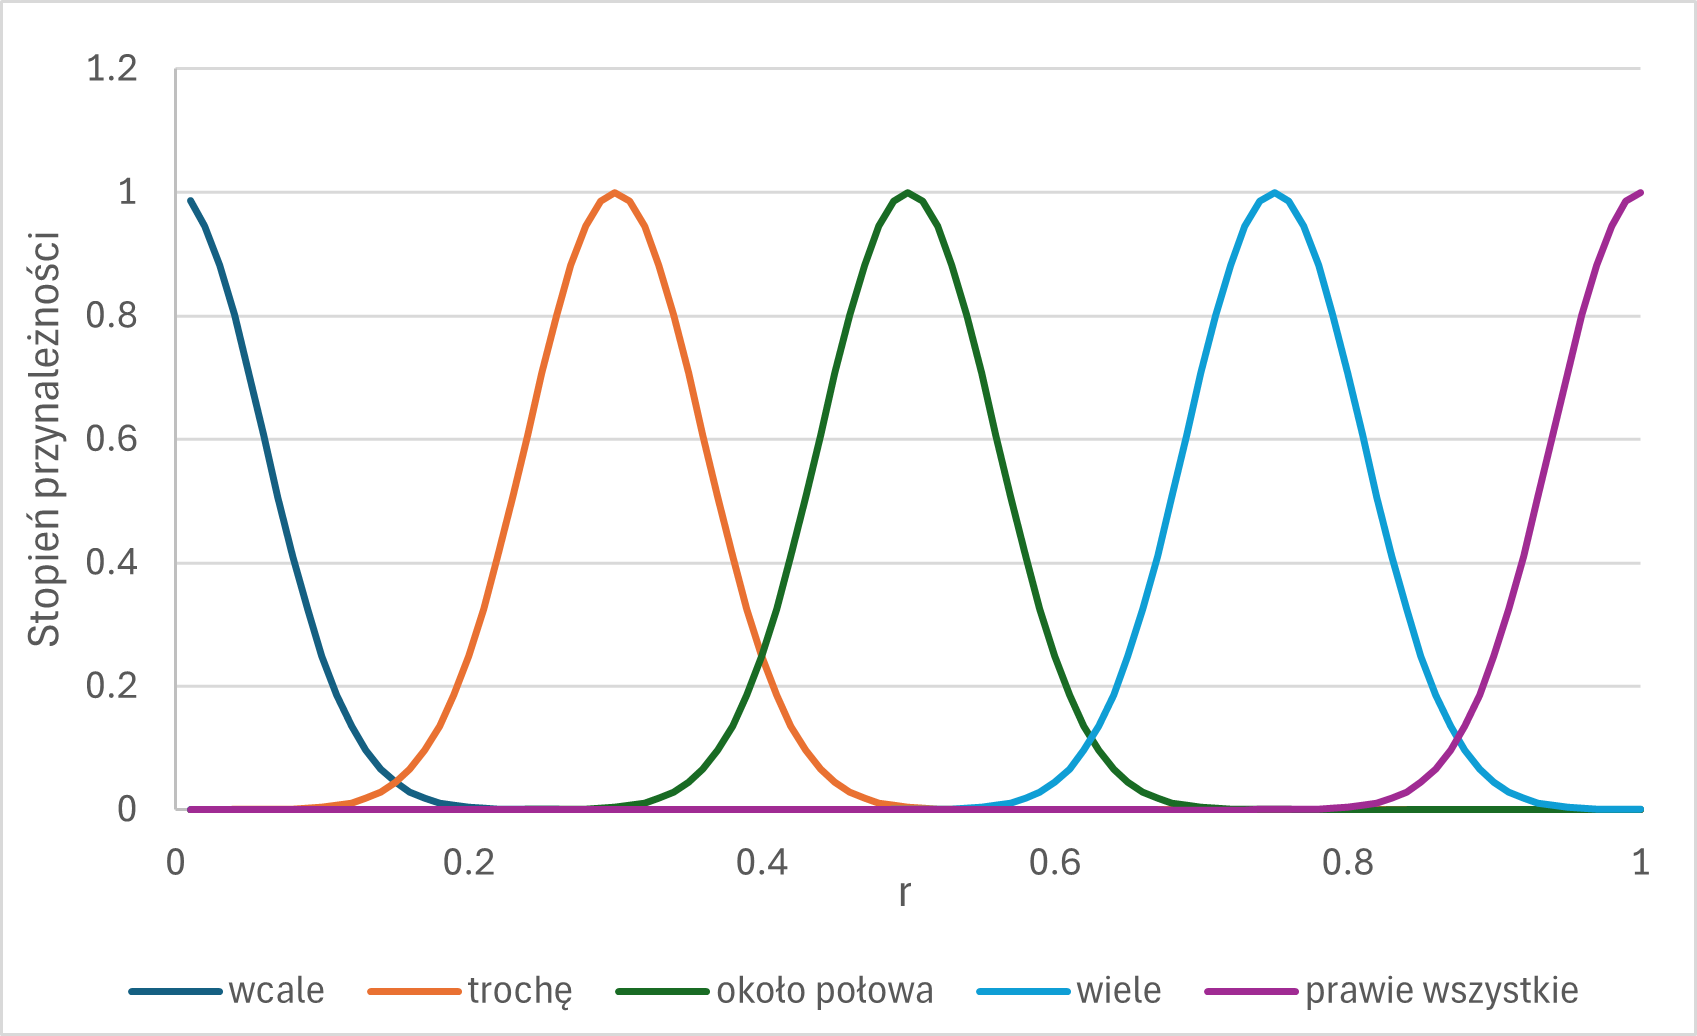
\includegraphics[width=0.7\textwidth]{img/a.png}
    \caption{Wykres funkcji przynależności dla kwantyfikatorów}
\end{figure}



\section{Narzędzia obliczeniowe: wybór/implementacja. Diagram UML klas do obliczeń rozmytych i generowania podsumowań}
Program został napisany w języku Java w wersji JDK 24. Do obsługi relacyjnej bazy danych PostgreSQL wykorzystano framework Spring Boot, który umożliwia wygodną konfigurację połączenia z bazą danych. Kod źródłowy komponentu odpowiedzialnego za obliczenia rozmyte został umieszczony w pakiecie o nazwie \texttt{fuzzy}. Znajduje sie w nim podstawowy model reprezentujący zbiory rozmyte, którego centralnym elementem jest abstrakcyjna klasa \texttt{FuzzySet}, która definiuje fundamentalne operacje na zbiorach rozmytych. Klasa ta udostępnia metody pozwalające na obliczanie podstawowych właściwości zbioru rozmytego, m.in. takich jak kardynalność oraz nośnik. Na bazie klasy \texttt{FuzzySet} zbudowane zostały trzy klasy reprezentujące konkretne typy funkcji przynależności: \texttt{GaussianFunction}, \texttt{TrapezoidalFunction} oraz \texttt{TriangularFunction}. Każda z tych klas implementuje matematyczną funkcję przynależności o charakterystycznym kształcie: odpowiednio gaussowskim, trapezoidalnym i trójkątnym. Dzięki temu możliwe jest precyzyjne modelowanie różnych pojęć językowych. \\
Oprócz modelu zbiorów rozmytych, pakiet \texttt{fuzzy} zawiera również klasy odpowiedzialne za tworzenie i przetwarzanie podsumowań lingwistycznych. Klasa \texttt{LinguisticVariable} reprezentuje zmienną lingwistyczną, która zawiera nazwę, przestrzeń rozważań oraz zestaw powiązanych z nią terminów lingwistycznych, np. „bardzo zimno”, „ciepło”, „gorąco”, które są reprezentowane przez odpowiednie zbiory rozmyte.
W strukturze podsumowań lingwistycznych wyróżniamy także kwalifikatory i sumaryzatory, które mają bardzo podobną strukturę, ponieważ są złożone z nazwy oraz przypisanego im zbioru rozmytego. Ich różnice wynikają jedynie z zastosowania, w jaki sposób są wykorzystywane w podsumowaniach lingwistycznych. W celu zachowania przejrzystości i uniknięcia duplikacji kodu, stworzona została wspólna klasa bazowa \texttt{LinguisticTerm}. 
Klasa \texttt{Quantifier} odpowiada za reprezentację kwantyfikatorów, takich jak „około połowy” czy „prawie żaden”. Kwantyfikator opisany jest za pomocą nazwy, funkcji przynależności oraz typu — może być kwantyfikatorem absolutnym lub względnym.
Kolejnym elementem pakietu jest klasa \texttt{SingleSubjectSummary}. To ona odpowiada za generowanie jednopodmiotowych podsumowań lingwistycznych oraz obliczanie miar jakości na podstawie przekazanych obiektów: sumaryzatora, kwalifikatora oraz kwantyfikatora. \\
Ostanim elementem jest klasa \texttt{DoubleSubjectSummary}, która generuje dwupodmiotowe podsumowania lingwistyczne wraz z ich miarami. \\
Strukturę logiczną opisanych klas oraz zależności między nimi przedstawiono diagramie UML dostępnym w załączniku lingustic.png.



\section{ Jednopodmiotowe podsumowania lingwistyczne. Miary jakości, podsumowanie optymalne}
Poniżej zaprezentowano wyniki eksperymentów polegających na generowaniu jednopodmiotowych podsumowań lingwistycznych. Eksperymenty zostały podzielone na trzy części. W każdym eksperymencie wykorzystano tylko kwalifikator relatywny. Dla każdego utworzonego podsumowania lingwistycznego obliczane były miary jakości oraz miara podsumowania optymalnego, które pozwala ocenić ostateczną miarę jakości podsumowania. W każdej z poniższych sekcji w tabelach przedstawiono wybrane podsumowania z wartością miary \textit{degree of truth} (\(T_1\)), która dla danego kwantyfikatora była większa niż 0{,}80 lub mniejsza od 0{,}20. Dodatkowo w tabeli zawarto wartości miary optymalnej, która jest obliczana na podstawie sumy iloczynów wag i wartości pozostałych miar (\(T_1\)–\(T_{11}\)). Pozostałe miary jakości zostały załączone w pliku \textit{Załącznik3.pdf}. W celu obliczenia miary podsumowania optymalnego przyjęto następujące wagi: \(w1 = 0.30\), \(w2 = 0.07\), \(w3 = 0.07\), \(w4 = 0.07\), \(w5 = 0.07\), \(w6 = 0.07\), \(w7 = 0.07\), \(w8 = 0.07\), \(w9 = 0.07\), \(w_{10} = 0.07\), \(w_{11} = 0.07\).


\subsection{Podsumowania lingwistyczne pierwszego typu}
W tej sekcji zostały przedstawione wyniki dla podsumowań lingwistycznych z jednym sumaryzatorem. Natomiast w tabeli nr.2 przedstawiono miary jakości oraz miarę podsumowania optymalnego dla podsumowania lingwistycznego nr.1 z tabeli nr.1:  \(T_1\) – degree of truth, \(T_2\) – degree of imprecision, \(T_3\) – degree of covering, \(T_4\) – degree of appropriateness, \(T_5\) – length of summary, \(T_6\) – degree of quantifier imprecision, \(T_7\) – degree of quantifier cardinality, \(T_8\), \(T_9\) - degree of qualifier imprecision, \(T_{10}\) - degree of qualifier cardinality, \(T_{11}\), \(T\) - miara podsumowania optymalnego. Znaczenia wartości odpowiednich miar zostały opisane w sekcji 6.1.

\begin{table}[H]
    \centering
    \normalsize
    \begin{tabular}{|c|p{8cm}|c|c|}
    \hline
    \textbf{Lp.} &\textbf{Podsumowanie} & \textbf{\(T_1\)} & \textbf{T} \\ \hline
    1. & Trochę pomiarów  jest/ma popołudniową godzinę & 0.92 & 0.55 \\ \hline
    2. & Około połowy pomiarów jest/ma umiarkowany wiatr & 0.89 & 0.53 \\ \hline
    3. & Prawie żaden pomiarów jest/ma bardzo silny waitr & 0.99 & 0.61 \\ \hline
    4. & Prawie żaden pomiarów jest/ma słaba widoczność & 0.86 & 0.56 \\ \hline
    5. & Około połowy pomiarów  jest/ma normalne zanieczyszczenie CO2 & 0.84 & 0.51 \\ \hline
    6. & Trochę pomiarów jest/ma bardzo dobra jakość powietrza & 1.00 & 0.57 \\ \hline
    7. & Prawie żaden pomiarów jest/ma suche powietrze & 0.05 & 0.31 \\ \hline
    8. & Wiele pomiarów  jest/ma umiarkowana widoczność & 0.02 & 0.22 \\ \hline
    9. & Prawie żaden pomiarów jest/ma bardzo wysokie UV & 0.06 & 0.32 \\ \hline
    10. & Prawie żaden pomiarów jest/ma dobra jakość powietrza & 0.01 & 0.30 \\ \hline 


    \end{tabular}
    \caption{Wyniki jednopodmiotowych podsumowań lingwistycznych typu 1 z \textit{degree of truth} oraz miarą optymalną.}
\end{table}

  \begin{table}[H]
    \centering
    \begin{tabular}{|c|c|c|c|c|c|c|c|c|c|c|c|}
    \hline
    \textbf{\(T_1\)} &\textbf{\(T_2\)} & \textbf{\(T_3\)} & \textbf{\(T_4\)} & \textbf{\(T_5\)} & \textbf{\(T_6\)} & \textbf{\(T_7\)} & \textbf{\(T_8\)} & \textbf{\(T_9\)} & \textbf{\(T_{10}\)} & \textbf{\(T_{11}\)} & \textbf{\(T\)} \\ \hline
    0.92 & 0.62 & 0.37 & 0.00 & 1.00 & 0.65 & 0.43 & 0.76 & 0.00 & 0.00 & 0.00 & 0.55 \\ \hline
    \end{tabular}
    \caption{Miary jakości dla podsumowania nr. 1 z tabeli nr.1.}
\end{table}  

\subsection{Podsumowania lingwistyczne pierwszego typu z dwoma sumaryzatorami}
W tej sekcji zostały przedstawione wyniki dla podsumowań lingwistycznych z dwoma sumaryzatorami. 
W tabeli nr.4 przedstawiono miary jakości oraz miarę podsumowania optymalnego dla podsumowania lingwistycznego nr.4 z tabeli nr.3. Wszystkie miary zostały opisane w sekcji 6.1.


\begin{table}[H]
\begin{center}
\normalsize % lub \Large, \normalsize, itp.
\begin{tabular}{|c|p{8cm}|c|c|} % p{10cm} = zawijanie tekstu, szerokość dostosuj
\hline
\textbf{Lp.} & \textbf{Podsumowanie} & \textbf{\(T_1\)} & \textbf{T} \\ \hline
1. & Około połowy pomiarów  jest/ma normalne zanieczyszczenie CO2 i jest/ma normalne zanieczyszczenie NO2 & 0.81 & 0.45 \\ \hline
2. & Około połowy pomiarów  jest/ma wilgotne powietrze i jest/ma normalne ciśnienie  & 0.96 & 0.49 \\ \hline 
3. & Prawie żaden pomiarów jest/ma wieczorną godzinę i jest/ma dobrą widoczność & 0.99 & 0.55 \\ \hline
4. & Około połowy pomiarów  jest/ma umiarkowany wiatr i jest/ma normalne ciśnienie  & 0.94 & 0.49 \\ \hline
5. & Trochę pomiarów jest/ma popołudniowa godzinę i jest/ma normalne ciśnienie  & 0.90 & 0.47 \\ \hline
6. & trochę pomiarów  jest/ma bardzo dobra jakość powietrza i jest/ma normalne zanieczyszczenie CO2 & 0.99 & 0.50 \\ \hline 
7. & Około połowy pomiarów  jest/ma umiarkowane powietrze i jest/ma normalne zanieczysczenie NO2 & 0.03 & 0.22 \\ \hline
8. & Około połowy pomiarów  jest/ma słaby wiatr i jest/ma umiarkowaną widoczność & 0.18 & 0.26 \\ \hline
9. & Około połowy pomiarów  jest/ma ciepła temperaturę i jest/ma umiarkowany wiatr & 0.06 & 0.23 \\ \hline 
10. & Trochę pomiarów jest/ma wysokie zanieczyszczenie CO2 i jest/ma normalne zanieczyszczenie NO2 & 0.12 & 0.23 \\ \hline
11. & Trochę pomiarów jest/ma ciepła temperaturę i jest/ma niskie UV & 0.03 & 0.21 \\ \hline
12. & Prawie żaden pomiarów jest/ma poranna godzinę i jest/ma wilgotne powietrze & 0.01 & 0.25 \\ \hline
\end{tabular}
\caption{Wyniki jednopodmiotowych podsumowań lingwistycznych typu 1 z dwoma sumaryzatorami z miarą \textit{degree of truth} oraz miarą optymalną.}
\end{center}
\end{table}

\begin{table}[H]
    \centering
    \begin{tabular}{|c|c|c|c|c|c|c|c|c|c|c|c|}
    \hline
    \textbf{\(T_1\)} &\textbf{\(T_2\)} & \textbf{\(T_3\)} & \textbf{\(T_4\)} & \textbf{\(T_5\)} & \textbf{\(T_6\)} & \textbf{\(T_7\)} & \textbf{\(T_8\)} & \textbf{\(T_9\)} & \textbf{\(T_{10}\)} & \textbf{\(T_{11}\)} & \textbf{\(T\)} \\ \hline
    0.94 & 0.01 & 0.99 & 0.00 & 0.50 & 0.60 & 0.62 & 0.29 & 0.00 & 0.00 & 0.00 & 0.49 \\ \hline
    \end{tabular}
    \caption{Miary jakości dla podsumowania nr. 4 z tabeli nr.3.}
\end{table}  


\subsection{Podsumowania lingwistyczne drugiego typu z jednym sumaryzatorem}
W tej sekcji zostały przedstawione wyniki dla podsumowań lingwistycznych z jednym sumaryzatorem i jednym kwalifikatorem. W tabeli nr.6 przedstawiono miary jakości oraz miarę podsumowania optymalnego dla podsumowania lingwistycznego nr.10 z tabeli nr.5. Wszystkie przedstawione w niej miary zostały opisane w sekcji 6.1. 


\begin{table}[H]
\begin{center}
\normalsize % lub \Large, \normalsize, itp.
\begin{tabular}{|c|p{8cm}|c|c|} % p{10cm} = zawijanie tekstu, szerokość dostosuj
\hline
\textbf{Lp.} & \textbf{Podsumowanie} & \textbf{\(T_1\)} & \textbf{T} \\ \hline
1. & Prawie żaden pomiarów będący/mający wieczorna godzinę jest/ma bardzo silny wiatr & 1.0 & 0.81 \\ \hline
2. & Trochę pomiarów będący/mający ekstremalne UV jest/ma dobra jakość powietrza & 0.84 & 0.74 \\ \hline
3. & Około połowy pomiarów będący/mający południowa godzinę jest/ma słaby wiatr & 0.99 & 0.70 \\ \hline
4. & Prawie wszystkie pomiarów będący/mający gorąca temperaturę jest/ma normalne zanieczysczenie NO2 & 0.86 & 0.70 \\ \hline
5. & Prawie wszystkie pomiarów będący/mający normalne zanieczyszczenie CO2 jest/ma normalne zanieczysczenie NO2 & 0.99 & 0.67 \\ \hline
6. & Wiele pomiarów będący/mający ekstremalne UV jest/ma południowa godzinę & 0.20 & 0.57 \\ \hline
7. & Prawie wszystkie pomiarów będący/mający niezdrowe zanieczysczenie CO2 jest/ma normalne zanieczyszczenie NO2 & 0.01 & 0.45 \\ \hline
8. & Wiele pomiarów będący/mający niskie UV jest/ma umiarkowana widoczność & 0.09 & 0.41 \\ \hline
9. & Wiele pomiarów będący/mający wieczorna godzinę jest/ma słaby wiatr & 0.16 & 0.51 \\ \hline
10. & Około połowy pomiarów będący/mający wilgotne powietrze jest/ma umiarkowana temperaturę & 0.08 & 0.43 \\ \hline 
\end{tabular}
\caption{Wyniki jednopodmiotowych podsumowań lingwistycznych typu 2 z miarą \textit{degree of truth} oraz miarą optymalną.}
\end{center}
\end{table}


\begin{table}[H]
    \centering
    \begin{tabular}{|c|c|c|c|c|c|c|c|c|c|c|c|}
    \hline
    \textbf{\(T_1\)} &\textbf{\(T_2\)} & \textbf{\(T_3\)} & \textbf{\(T_4\)} & \textbf{\(T_5\)} & \textbf{\(T_6\)} & \textbf{\(T_7\)} & \textbf{\(T_8\)} & \textbf{\(T_9\)} & \textbf{\(T_{10}\)} & \textbf{\(T_{11}\)} & \textbf{\(T\)} \\ \hline
    0.08 & 0.49 & 0.57 & 0.06 & 1.00 & 0.60 & 0.62 & 0.71 & 0.32 & 0.50 & 1.00 & 0.43 \\ \hline
    \end{tabular}
    \caption{Miary jakości dla podsumowania nr. 10 z tabeli nr.5.}
\end{table}  


\section{Wielopodmiotowe podsumowania lingwistyczne i~ich miary jakości} 
Poniżej zaprezentowano wyniki eksperymentów polegających na generowaniu wielopodmiotowych podsumowań lingwistycznych. Z bazy danych opisanej w sekcji 2.1 zostały wyodrębnione cztery podmioty, które dzielą podmiot główny - pomiar, na pomiar wykonany na danym kontynencie. Wyróżnione zostały cztery kontynenty - Europe, Asia, Africa, America (opisuje jednocześnie Amerykę Południową i Północną). Podsumownania wielopodmiotowe będą generowane w czterech formach, ograniczając się przy tym do wykorzystania w tym samym momencie tylko dwóch podmiotów. W tabelach zaprezentowano treść podsumowania oraz wartość miary degree of truth, która za każdym razem opisuje prawdziwość danego wyrażenia.

\subsection{Dwupodmiotowe podsumowania w pierwszej formie}
W tej sekcji zostały przedstawione wyniki dla dwupodmiotowych podsumowań lingwistycznych z jednym sumaryzatorem.

\begin{table}[H]
\begin{center}
\normalsize % lub \Large, \normalsize, itp.
\begin{tabular}{|c|p{10cm}|c|} % p{10cm} = zawijanie tekstu, szerokość dostosuj
\hline
\textbf{Lp.} & \textbf{Podsumowanie} & \textbf{\(T_1\)} \\ \hline
1. & Prawie żaden pomiarów z Africa w porównaniu do pomiarów z America jest/ma bardzo zimna temperature & 1.0 \\\hline
2. & Prawie żaden pomiarów z Asia w porównaniu do pomiarów z Africa jest/ma poranna godzinę & 0.96 \\\hline
3. & Prawie żaden pomiarów z America w porównaniu do pomiarów z Asia jest/ma suche powietrze & 0.85 \\\hline
4. & Trochę pomiarów z Asia w porównaniu do pomiarów z Europe jest/ma umiarkowana temperaturę & 0.95 \\\hline
5. & Trochę pomiarów z Europe w porównaniu do pomiarów z America jest/ma bardzo zimna temperaturę & 0.95 \\\hline
6. & Prawie żaden pomiarów z Europe w porównaniu do pomiarów z America jest/ma niezdrowe zanieczysczenie CO2  & 0.03 
\\\hline
7. & Trochę pomiarów z Africa w porównaniu do pomiarów z Europe jest/ma bardzo silny wiatr & 0.11 \\ \hline
8. & Około połowy pomiarów z Africa w porównaniu do pomiarów z Europe jest/ma wieczorna godzinę & 0.07 \\ \hline
9. & Wiele pomiarów z Africa w porównaniu do pomiarów z Europe jest/ma niezdrowe zanieczyszczenie CO2 & 0.04 \\ \hline 
10 & Prawie wszystkie pomiarów z Europe w porównaniu do pomiarów z America jest/ma wysokie cieśnienie & 0.05 \\ \hline
\end{tabular}
\caption{Wyniki dwupodmiotowych podsumowań lingwistycznych w pierwszej formie z miarą \textit{degree of truth}.}
\end{center}
\end{table}

\subsection{Dwupodmiotowe podsumowania w drugiej formie}
W tej sekcji zostały przedstawione wyniki dla dwupodmiotowych podsumowań lingwistycznych w drugiej formie.

\begin{table}[H]
\begin{center}
\normalsize % lub \Large, \normalsize, itp.
\begin{tabular}{|c|p{10cm}|c|} % p{10cm} = zawijanie tekstu, szerokość dostosuj
\hline
\textbf{Lp.} & \textbf{Podsumowanie} & \textbf{\(T_1\)} \\ \hline
1. & Prawie żaden pomiarów z Asia w porównaniu do pomiarów z Africa, które są/mają niezdrowe zanieczyszczenie CO2 jest/ma poranna godzinę & 0.96 \\\hline  
2. & Trochę pomiarów z Asia w porównaniu do pomiarów z Europe, które są/mają niezdrowe zanieczyszczenie CO2 jest/ma południowa godzinę & 0.83 \\\hline 
3. & Wiele pomiarów z Europe w porównaniu do pomiarów z Asia, które są/mają wilgotne powietrze jest/ma zimna temperature & 1.0 \\ \hline 
4. & Około połowy pomiarów z Europe w porównaniu do pomiarów z Asia, które są/mają wilgotne powietrze jest/ma ciepła temperaturę & 0.02 \\ \hline
5. & Wiele pomiarów z America w porównaniu do pomiarów z Africa, które są/mają normalne zanieczyszczenie NO2 jest/ma niebezpieczne zanieczyszczenie CO2 & 0.04 \\ \hline
6. & Trochę pomiarów z America w porównaniu do pomiarów z Africa, które są/mają zimna temperaturę jest/ma umiarkowany & 0.06 \\ \hline 
\end{tabular}
\caption{Wyniki dwupodmiotowych podsumowań lingwistycznych w drugiej formie z miarą \textit{degree of truth}.}
\end{center}
\end{table}

\subsection{Dwupodmiotowe podsumowania w trzeciej formie}
W tej sekcji zostały przedstawione wyniki dla dwupodmiotowych podsumowań lingwistycznych w trzeciej formie.

\begin{table}[H]
\begin{center}
\normalsize % lub \Large, \normalsize, itp.
\begin{tabular}{|c|p{10cm}|c|} % p{10cm} = zawijanie tekstu, szerokość dostosuj
\hline
\textbf{Lp.} & \textbf{Podsumowanie} & \textbf{\(T_1\)} \\ \hline
1. & Trochę pomiarów z Africa, które są/mają słaby wiatr, w porównaniu do pomiarów z Europe jest/ma niskie UV & 1.0 \\\hline
2. & Około połowy pomiarów z Asia, które są/mają wilgotne powietrze, w porównaniu do pomiarów z Africa jest/ma wysokie UV & 0.96 \\\hline
3. & Prawie wszystkie pomiarów z Asia, które są/mają wilgotne powietrze, w porównaniu do pomiarów z Europe jest/ma bardzo dobra jakość powietrza & 0.91 \\\hline
4. & Prawie wszystkie pomiarów z America, które są/mają wysokie UV, w porównaniu do pomiarów z Africa jest/ma umiarkowana widoczność & 0.12 \\ \hline
5. & Prawie żaden pomiarów z Europe, które są/mają niezdrowe zanieczysczenie NO2, w porównaniu do pomiarów z Asia jest/ma bardzo zimna temperaturę & 0.01 \\ \hline
6. & Trochę pomiarów z America w porównaniu do pomiarów z Africa, które są/mają zimna temperaturę jest/ma umiarkowany wiatr & 0.06 \\ \hline
\end{tabular}
\caption{Wyniki dwupodmiotowych podsumowań lingwistycznych w trzeciej formie z miarą \textit{degree of truth}.}
\end{center}
\end{table}

\subsection{Dwupodmiotowe podsumowania w czwartej formie}
W tej sekcji zostały przedstawione wyniki dla dwupodmiotowych podsumowań lingwistycznych w czwartej formie.

\begin{table}[H]
\begin{center}
\normalsize % lub \Large, \normalsize, itp.
\begin{tabular}{|c|p{10cm}|c|} % p{10cm} = zawijanie tekstu, szerokość dostosuj
\hline
\textbf{Lp.} & \textbf{Podsumowanie} & \textbf{\(T_1\)} \\ \hline
1. & Więcej pomiarów z Europe niż pomiarów z Asia jest/ma umiarkowana temperaturę & 0.50 \\\hline
2. & Więcej pomiarów z Asia niż pomiarów z Europe jest/ma umiarkowana temperaturę & 0.64 \\\hline
3. & Więcej pomiarów z America niż pomiarów z Europe jest/ma południowa godzinę & 0.81 \\\hline
4. & Więcej pomiarów z Europe niż pomiarów z America jest/ma południowa godzine & 0.43 \\\hline
5. & Więcej pomiarów z America niż pomiarów z Europe jest/ma niskie UV & 0.73 \\\hline
6. & Więcej pomiarów z Europe niż pomiarów z America jest/ma niskie UV & 0.43 \\\hline 
\end{tabular}
\caption{Wyniki dwupodmiotowych podsumowań lingwistycznych w czwartej formie z miarą \textit{degree of truth}.}
\end{center}
\end{table}

\section{Dyskusja, wnioski}

\subsection{Jednopodmiotowe podsumowania lingwistyczne}
W pierwszym doświadzeniu zwiazanym z generowaniem jednopodmiotowych podsumowań lingwistycznych wygenerowano podsumowania pierwszego typu z jednym sumaryzatorem. Dla każdej zmiennej lingwistycznej stworzono podsumowania ze wszystkimi dostępnymi kwantyfikatorami, jednak szczególna uwaga została poświęcona podsumowaniom o najwyższej i najniższej jakości — ocenianej za pomocą miary \( T_1 \), będącej stopniem prawdziwości podsumowania. Z przeprowadzonych doświadczeń wynika, że częściej pojawiały się podsumowania z kwantyfikatorami typu \textit{„prawie żaden”} lub \textit{„trochę”} niż z kwantyfikatorami \textit{„wiele”} czy \textit{„prawie wszystkie”}. Wskazuje to na fakt, że wiele właściwości pojawiających się w bazie danych występowało stosunkowo rzadko. Przykłady takich cech to \textit{„słaba widoczność”} czy \textit{„dobra jakość powietrza”}. Tym samym system podsumowań trafnie odzwierciedla statystyczną rzadkość tych zjawisk w danych.
Wysoka wartość miary \( T_1 \) — jak np. w podsumowaniu \textit{„Trochę pomiarów jest/ma popołudniową godzinę”} (\( T_1 = 0{,}92 \)) — wskazuje na dużą zgodność wygenerowanego podsumowania z rzeczywistymi danymi. Jednak, jak pokazują dodatkowe miary, taka zgodność nie zawsze oznacza wysoką ogólną jakość podsumowania. Dla tego konkretnego przykładu inne miary wskazują na różne aspekty jakości: Wartości miar jakości dla tego podsumowania to: \( T_2 = 0{,}62 \) (umiarkowana precyzja sumaryzatora), \( T_3 = 0{,}37 \) (około 1/3 pomiarów spełnia warunki podsumowania, zgodnie z użytym kwantyfikatorem \textit{„trochę”}), \( T_4 = 0{,}00 \) (związane z tylko jednym sumaryzatorem), \( T_5 = 1{,}00 \) (dokładnie jeden sumaryzator został wykorzystany), \( T_6 = 0{,}65 \) (dobra precyzja kwantyfikatora), \( T_7 = 0{,}43 \) (umiarkowana liczność obiektów spełniających warunki), \( T_8 = 0{,}76 \) (sumaryzator słabo odwzorowuje dane), a \( T_9 = T_{10} = T_{11} = 0{,}00 \) wskazują na brak kwalifikatora w podsumowaniu.
Ostateczna miara jakości podsumowania, oznaczona jako \( T \), wynosi \( 0{,}55 \), co sugeruje średnią jakość wygenerowanego podsumowania, mimo wysokiego stopnia prawdziwości.
Natomist podsumowanie \textit{"Wiele pomiarów jest/ma umiarkowana widoczność"} z miarą \(T_1\) = (0,02) oznacza, że te zdanie jest prawie całkowicie nieprawdziwe i tylko bardzo niewielka część danych ma umiarkowaną widoczność.

% Wniosek z tej analizy jest taki, że nawet przy wysokim \( T_1 \), inne miary mogą wskazywać na ograniczenia jakościowe danego podsumowania — szczególnie, gdy sumaryzator jest słabo dopasowany do danych lub gdy brak kwalifikatora obniża precyzję kontekstu. Dodatkowo należy zauważyć, że najgorsze podsumowania (np. z \( T_1 < 0{,}1 \)) często dotyczyły rzadko występujących cech, takich jak \textit{„dobra jakość powietrza”} czy \textit{„bardzo wysokie UV”}, co podkreśla znaczenie częstotliwości cechy w danych jako czynnika wpływającego na jakość wygenerowanego podsumowania.

W drugim doświadczeniu tworzono podsumowania z wykorzystaniem dwóch sumaryzatorów. Podobnie jak w przypadku pierwszego doświadczenia, jednak w tym przypadku dużo większa część wszystkich podsumowań lingwistycznych była oznaczona przez kwantyfikator \textit{"prawie żaden"} lub \textit{"trochę"}. Jest to związane z tym, że dużo ciężej stworzyć takie podsumowanie, które odpowiada jednocześnie dwóm cechom. Na wszystkie możliwe kombinacje podsumowań lingwistycznych z dwoma sumaryzatorami tylko 6 posiadało kwantyfikator \textit{"prawie wszystkie"} lub \textit{"wiele"}. Warte wspomnienia jest tutaj m.in. zdanie \textit{"Około połowy pomiarów jest/ma normalne zanieczyszczenie CO2 i jest/ma normalne zanieczyszczenie NO2"}, które niesie bardzo konkretną informację o dobrych warunkach atmosferycznych dotyczących zanieczyszczeń powietrza. Warte uwagi jest zdanie \textit{"Prawie żaden pomiarów jest/ma wieczorną godzinę i jest/ma dobrą widoczność"}, które jest bardzo logicznym zdaniem, ponieważ zwykle w wieczornych godzinach, kiedy jest ciemno, to widoczność jest ograniczona. Miary jakości dla zdania \textit{„Około połowy pomiarów jest/ma normalne ciśnienie i jest/ma umiarkowany wiatr”} przedstawione w tabeli nr. 4 niosą ze sobą następujące informacje. \(T_1\) = (0.94) czyli to podsumowanie jest bardzo zgodne z tym, co reprezentują dane w bazie danych. Następnie \(T_2\) = (0.01) sugeruje że obydwa sumaryzatory \textit{"normalne ciśnienie powietrza"} oraz \textit{"umiarkowany wiatr"} są bardzo precyzyjnie określone. \(T_3\) = (0.99) miara która oznacza, że znaczna część danych spełnia warunki podsumowania. \(T_4\) =  (0.00). \(T_5\) = (0.5) - dwa sumaryzatory w jednym podsumowaniu. \(T_6\) = (0.6), wykorzystywany kwantyfikator \textit{"około połowy"} jest nieco mniej precyzyjny w porównaniu do kwantyfikatora opisanego w poprzednim doświadczeniu (\textit{"trochę"} miał \(T_6\) = (0.65)). \(T_7\) = (0.62) oznacza umiarkowaną liczebność obiektów w kwantyfikatorze wykorzystanym w tym podsumowaniu. \(T_8\) = (0.29), wykorzystane sumaryzatory dobrze odpowiadają danym zawartym w bazie danych. Miary \(T_9\), \(T_{10}\) i \(T_{11}\) są równe (0.00), ponieważ podsumowanie nie zawiera kwalifikatora. Ostateczna miara jakości podsumowania (\(T\)) wynosi (0{.}49), i jest nieco gorsza niż ta w przypadku przykładu podsumownia lingwistycznego z jednym sumaryzatorem. \\
W kolejnym eksperymencie analizowano jednopodmiotowe podsumowania lingwistyczne drugiego typu, które zawierają zarówno kwalifikator, jak i sumaryzator. Dla każdej możliwej kombinacji kwalifikatora z sumaryzatorem wygenerowano odpowiednie podsumowania. W przeciwieństwie do podsumowań pierwszego typu, tutaj liczba wygenerowanych podsumowań dla poszczególnych kwantyfikatorów była bardziej wyrównana — np. dla kwantyfikatora \textit{"wiele"} uzyskano aż 116 podsumowań. Wynika to z faktu, że podsumowania drugiego typu nie opisują ogólnych cech całego zbioru danych, lecz skupiają się jedynie na tych rekordach, które spełniają warunki kwalifikatora. Dla przykładu, w zdaniu \textit{"Wiele pomiarów będący/mający ekstremalne UV jest/ma południowa godzinę"} rozpatrywane są wyłącznie te obserwacje, które spełniają warunek \textit{"ekstremalne UV"}.
Miary jakości dla podsumowania nr 10: \textit{"Około połowy pomiarów będący/mający wilgotne powietrze jest/ma umiarkowana temperaturę"} ujawnia niższą jakość podsumowania. Wartość \(T_1 = 0{,}08\) świadczy o bardzo niskiej zgodności danych z podsumowaniem, a umiarkowane wartości \(T_2 = 0{,}49\) i \(T_3 = 0{,}57\) sugerują przeciętną precyzję sumaryzatora i ograniczoną liczność danych spełniających warunki podsumowania. \(T_4\) = (0{,}06) oznacza, że większkość danych zawierających się w sumaryzatorze tworzy trafne podsumowanie. Miary \(T_6 = 0{,}60\) i \(T_7 = 0{,}62\) wskazują na umiarkowaną precyzję kwantyfikatora i liczność obiektów, natomiast \(T_8 = 0{,}71\) sugeruje, że sumaryzator nie oddaje dokładnie rzeczywistych danych. Niska wartość \(T_9 = 0{,}32\) wskazuje na stosunkowo precyzyjny kwalifikator, im mniejsza wartość tym lepiej. \(T_{10}\) = (0.50), co oznacza, że połowa obiektów jest objęte kwalifikatorem \textit{"wilgotne powietrze"}. \(T_{11}\) = (1.00), czyli w podsumowaniu został wykorzystany jeden kwalifikator. Ogólna jakość podsumowania oceniona miarą \(T = 0{,}43\) pozostaje niezadowalająca.

% Z powyższej analizy wynika, że jakość podsumowań lingwistycznych drugiego typu w dużym stopniu zależy od trafności dobranego kwalifikatora i sumaryzatora, a także ich zgodności z rozkładem rzeczywistych danych w zbiorze.

\subsection{Wielopodmiotowe podsumowania lingwistyczne}
Na początku tej sekcji warto wspomnieć, że w wielopodmiotowych podsumowaniach wykorzystywana jest wyłącznie miara \(T_1\). Miary T2–T11, opracowane z myślą o klasycznych podsumowaniach jednozbiorowych, nie znajdują zastosowania w tym kontekście. Wynika to z faktu, że wiele z tych miar opiera się na zależnościach wewnątrz jednego zbioru (np. pokrycie przez sumaryzator), które nie są bezpośrednio mierzalne ani interpretowalne w przypadku porównania wielu podmiotów. Wielopodmiotowe podsumowania lingwistyczne były generowane w czterech różnych formach. Pierwsza z nich dotyczyła podsumowania, w którym występują dwa podmioty i jeden sumaryzator. Przeprowadzone doświadczenie doprowadziło do ciekawych rezultatów, mianowicie w przeciwieństwie do jednopodmiotowych podsumowań lingwistycznych, liczba podsumowań wygenerowanych z miarą \(T_1\) większa od 0.01 dla kwantyfikatórów \textit{"prawie żaden"} oraz \textit{"trochę"} nie jest dominująca. W tym przypadku uzyskano najwięcej podsumowań dla kwantyfikatora \textit{"około połowy"}. Podział bazy danych na cztery podzbiory pozwolił na uzyskanie dużo bardziej szczegółowych informacji dotyczących pomiarów. Np. podsumowanie \textit{"Prawie żaden pomiarów z Africa w porównaniu do pomiarów z America jest/ma bardzo zimna temperature"} \(T_1 = 1.00\) potwierdza bardzo intuicyjne skojarzenie na temat temperatur, jakie występują  w Afryce i Ameryce. Natomiast podsumowanie \textit{"Prawie żaden pomiarów z America w porównaniu do pomiarów z Asia jest/ma suche powietrze"} nie jest od razu oczywiste, że klimat amerykański jest suchszy od azjatyckiego. \\
Podsumowania wielopodmiotowe w drugiej oraz trzeciej formie pozwalają na jeszcze większe uszczegółowienie informacji, jakie niosą ze sobą te podsumowania. Występuje tutaj kwalifikator, który dotyczy pierwszego albo drugiego podmiotu. Dzięki temu możliwe jest nie tylko porównanie dwóch różnych grup, ale również uwzględnienie określonej cechy charakteryzującej jedną z nich, co znacząco zwiększa wartość informacyjną takich podsumowań. W drugiej formie kwalifikator odnosi się do drugiego podmiotu. Przykładowo, podsumowanie: \textit{"Trochę pomiarów z Asia w porównaniu do pomiarów z Europe, które są/mają niezdrowe zanieczyszczenie CO2, jest/ma południową godzinę”} \(T_1 = 0.83\)
wskazuje, że tylko niewielka część pomiarów z Azji, w porównaniu do tych z Europy spełniających określony warunek niezdrowego zanieczyszczenia CO2, ma południową godzinę. Wartość stopnia prawdziwości na poziomie 0.83 świadczy o dość wysokiej zgodności tej informacji z danymi źródłowymi. Z kolei w trzeciej formie kwalifikator odnosi się do pierwszego podmiotu. Taka struktura pozwala określić, jaka część pierwszego podmiotu (z uwzględnieniem jego właściwości) różni się od drugiego. Przykład: \textit{"Prawie wszystkie pomiarów z Asia, które są/mają wilgotne powietrze, w porównaniu do pomiarów z Europe, jest/ma bardzo dobrą jakość powietrza”}. Miara \(T_1 = 0.91\) pokazuje, że większość pomiarów z Azji, w warunkach wilgotnego powietrza, ma lepszą jakość powietrza niż Europa i to z dużą zgodnością z obiektami z bazy danych. \\
Ostatnia - czwarta forma określa czy dany podmiot ma więcej elementów spełniających warunki danego sumaryzatora. Na podstawie przeprowadzonych doświadczeń otrzymano dla przykładu: \textit{"Więcej pomiarów z America niż pomiarów z Europe jest/ma południowa godzinę"} z miarą \(T_1 = 0.81\), która oznacza, że rzeczywiście pomiary dokonane w Ameryce przeważają liczebnością w aspekcie południowej godziny w stosunku do Europy. Jednak warto zwrócić uwagę na to samo zdanie ale z podmiotami zamienionymi miejscami: \textit{Więcej pomiarów z Europe niż pomiarów z America jest/ma południowa godzine}. Intuicja mogła by wskasywać, ze \(T_1\) powinno wyności (0.19), aby wartości zsumowały się do 1, jednak \(T_1\) = (0.43), co jest związane z tym, że porównywane są inne zbiory.

\subsection{Wnioski}
\begin{itemize}
    \item Miara \(T_1\) przekazuje najistotniejsze informacje na temat jakości generowanych podsumowań lingwistycznych. 
    % Doprecyzowanie, że chodzi o jakość.

    \item Podczas generowania jednopodmiotowych podsumowań lingwistycznych najczęściej pojawiają się te z kwantyfikatorem \textit{"prawie żaden"} lub \textit{"trochę"}.
    % Uproszczenie stylu + poprawa gramatyczna ("dużo częściej pojawią się te..." brzmi nienaturalnie)

    \item Znacznie trudniej jest wygenerować wysokiej jakości podsumowania spełniające dwie lub więcej cech (czyli złożone podsumowania z wieloma sumaryzatorami).
    % Dodano wyjaśnienie w nawiasie dla większej jasności

    \item Wartości stopnia przynależności dla kolejnych kwantyfikatorów powinny przecinać się w połowie, co zapewnia płynność i ciągłość rozkładu językowego.
    % Dodano wyjaśnienie: dlaczego to jest istotne?

    \item Podsumowania jednopodmiotowe drugiego typu pozwalają na uszczegółowienie informacji względem podsumowań pierwszego typu.
    % „w stosunku do” → „względem” — bardziej formalne i krótsze.

    \item Generowanie wielopodmiotowych podsumowań lingwistycznych umożliwia uzyskanie bardziej szczegółowych informacji poprzez porównania między podmiotami w zbiorze danych.
    % Poprawiono literówkę: "szczegółowychi"

    \item Podsumowania wielopodmiotowe, w przeciwieństwie do jednopodmiotowych, umożliwiają identyfikację zależności między podmiotami w badanym zbiorze danych.
    % "dają możliwość znalezienia zależności" → „umożliwiają identyfikację” — bardziej naukowy styl

    \item Poprawna definicja funkcji przynależności oraz dobór sumaryzatora znacząco wpływa na jakość uzyskanych podsumowań lingwistycznych.
\end{itemize}



\section{Braki w realizacji projektu 2.}
Wymienić wg opisu Projektu 2. wszystkie niezrealizowane obowiązkowe elementy projektu, ewentualnie
podać merytoryczne (ale nie czasowe) przyczyny tych braków. 


\begin{thebibliography}{99}
\bibitem{baza} World Weather Repository - kaggle, \url{https://www.kaggle.com/datasets/nelgiriyewithana/global-weather-repository?resource=download}. [dostęp 18.05.2025r.]
 \bibitem{niewiadomski19} A. Niewiadomski, Zbiory rozmyte typu 2. Zastosowania w reprezentowaniu informacji.  Seria „Problemy współczesnej informatyki” pod redakcją L. Rutkowskiego. Akademicka Oficyna Wydawnicza EXIT, Warszawa, 2019.
\bibitem{zadrozny06} S. Zadrożny, Zapytania nieprecyzyjne i lingwistyczne podsumowania baz danych, EXIT, 2006, Warszawa
\bibitem{niewiadomski08} A. Niewiadomski, Methods for the Linguistic Summarization of Data: Applications of Fuzzy Sets and Their Extensions, Akademicka Oficyna Wydawnicza EXIT, Warszawa, 2008.
\end{thebibliography}

\end{document}
